\subsubsection{CUDA} \label{background:graphical_processing_units:cuda}

CUDA \cite{cuda} is Nvidia's general purpose parallel computing platform and programming model that allows software engineers to leverage the parallel compute engines in Nvidia GPUs.
Although the CUDA software environment can be imported in several supported programming languages, development of GPU accelerated programs have traditionally been done in C++ with CUDA functionality imported through header files \cite{cuda}.

The CUDA programming model is designed to be utilized to solve parallel problems where the GPU is used.
To programmers, the programming model is made up of a hierarchy of three units of different granularity: \textit{threads}, \textit{blocks}, and \textit{grids}.

\paragraph{Threads, Blocks and Grids}
CUDA threads are the most granular units of parallelism in the CUDA programming model.
Thread blocks are collections of threads that can be either one-, two- or three-dimensional.
Grids are at the top of the hierarchy, as collections of thread blocks.
Both thread blocks and the grids can either be one-, two- or three-dimensional.
Thus, their dimensions are referred to as $x$ for width, $y$ for height and $z$ for depth.
In the CUDA model, each individual thread can be distinctly identified by its index in a thread block, and the thread block's index in a grid.
When developing parallel programs, each thread has direct access to its (up to) three-dimensional index inside its thread block, and its thread block's (up to) three-dimensional index in its grid.
If a thread resides in a three-dimensional thread block of dimensions $(Dx_b, Dy_b, Dz_b)$ at index $(x_b, y_b, z_b)$, its unique index within said block can be computed using:
\begin{equation}
  i_b = (x_b + y_bDx_b + z_bDx_bDy_b)
\end{equation}
Then, we can compute the thread's unique grid-wide index.
If the thread's thread block resides in a grid of dimensions $(Dx_g, Dy_g, Dz_g)$ at grid-index $(x_g, y_g, z_g)$, the thread's unique grid-wide index can be computed using:

\begin{equation}
  i_g = (x_g + y_gDx_g + z_gDx_gDy_g)(Dx_bDy_bDz_b) + i_b
\end{equation}

This thread-hierarchy provides a natural way to perform computations over elements in e.g. vectors, matrices or tensors.
All threads in a thread block must reside on the same \textit{stream multiprocessor core} in the GPU.
Therefore, there is a size limit on how large thread blocks can be.
The two types of Nvidia GPUs used in this thesis, the Nvidia Tesla V100 and the Nvidia GTX 1660 SUPER, have limits of 2048 and 1024 threads per thread block respectively.

\definecolor{devicecolor}{RGB}{220,255,255}
\definecolor{gridcolor}{RGB}{255,255,225}
\definecolor{blockcolor}{RGB}{255,200,200}
\definecolor{threadcolor}{RGB}{255,125,125}

\begin{figure}[H]
\begin{center}
\scalebox{0.75}{
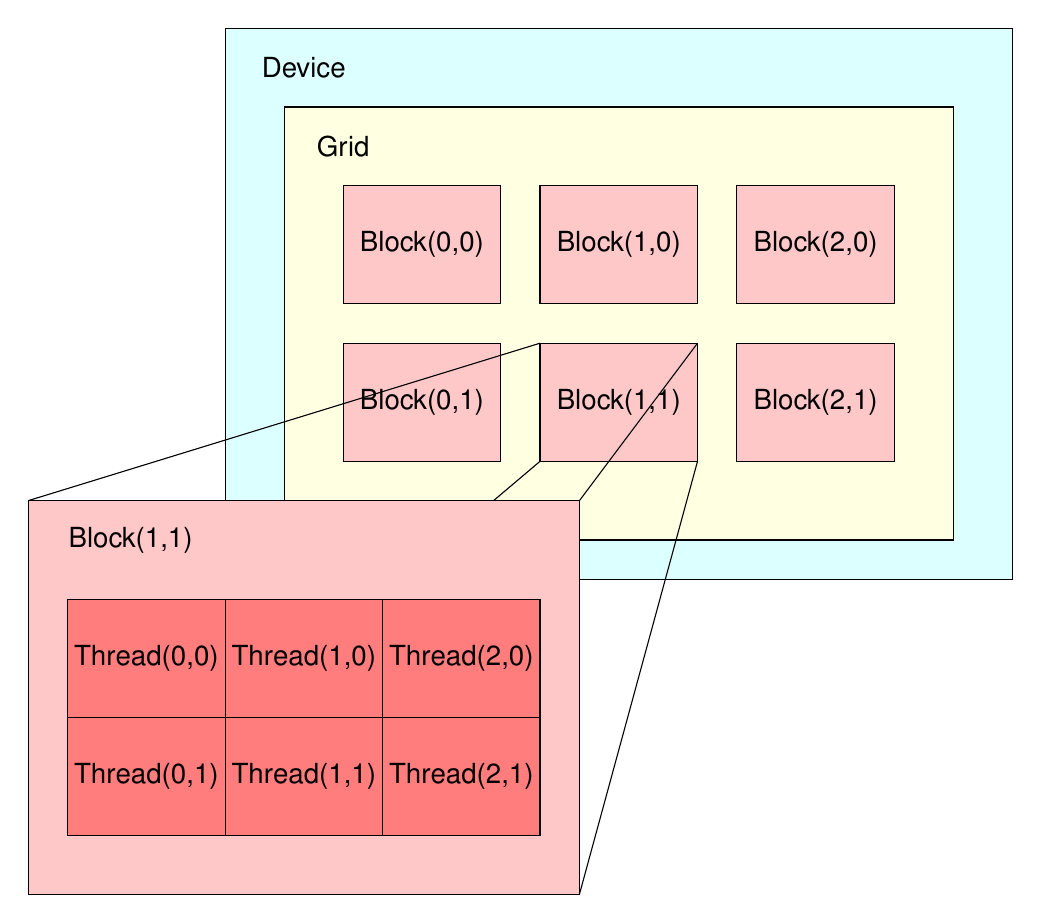
\begin{tikzpicture}
  % draw device rectangle
  \node at(0,0)[rectangle,draw,minimum width=10cm,minimum height=7cm,fill=devicecolor](device){};
  % draw "Device" text
  \node at(-4,3){\fontfamily{phv}\selectfont Device};
  % draw grid rectangle
  \node at(0,-.25)[rectangle,draw,minimum width=8.5cm,minimum height=5.5cm,fill=gridcolor](grid){};
  % draw "Grid" text
  \node at(-3.5,2){\fontfamily{phv}\selectfont Grid};
  % draw block rectangles inside grid rectangle
  \node at(-2.5,.75)[rectangle,draw,minimum width=2cm,minimum height=1.5cm,fill=blockcolor](block1){};
  \node at(0,.75)[rectangle,draw,minimum width=2cm,minimum height=1.5cm,fill=blockcolor](block2){};
  \node at(2.5,.75)[rectangle,draw,minimum width=2cm,minimum height=1.5cm,fill=blockcolor](block3){};
  \node at(-2.5,-1.25)[rectangle,draw,minimum width=2cm,minimum height=1.5cm,fill=blockcolor](block4){};
  \node at(0,-1.25)[rectangle,draw,minimum width=2cm,minimum height=1.5cm,fill=blockcolor](block5){};
  \node at(2.5,-1.25)[rectangle,draw,minimum width=2cm,minimum height=1.5cm,fill=blockcolor](block6){};
  % draw "Block(x,x)" text for each block
  \node at(-2.5,.75){\fontfamily{phv}\selectfont Block(0,0)};
  \node at(0,.75){\fontfamily{phv}\selectfont Block(1,0)};
  \node at(2.5,.75){\fontfamily{phv}\selectfont Block(2,0)};
  \node at(-2.5,-1.25){\fontfamily{phv}\selectfont Block(0,1)};
  \node at(0,-1.25){\fontfamily{phv}\selectfont Block(1,1)};
  \node at(2.5,-1.25){\fontfamily{phv}\selectfont Block(2,1)};
  % draw zoom lines to detailed block rectangle
  \draw (-1,-.5) -- (-7.5,-2.5);
  \draw (1,-.5) -- (-.5,-2.5);
  \draw (-1,-2) -- (-7.5,-7.5);
  \draw (1,-2) -- (-.5,-7.5);
  % draw detailed block rectangle
  \node at(-4,-5)[rectangle,draw,minimum width=7cm,minimum height=5cm,fill=blockcolor](detailedblock){};
  % draw "Block(1,1)" text for detailed block
  \node at(-6.2,-3){\fontfamily{phv}\selectfont Block(1,1)};
  % draw thread rectangles
  \node at(-6,-4.5)[rectangle,draw,minimum width=2cm,minimum height=1.5cm,fill=threadcolor](thread1){};
  \node at(-4,-4.5)[rectangle,draw,minimum width=2cm,minimum height=1.5cm,fill=threadcolor](thread2){};
  \node at(-2,-4.5)[rectangle,draw,minimum width=2cm,minimum height=1.5cm,fill=threadcolor](thread3){};
  \node at(-6,-6)[rectangle,draw,minimum width=2cm,minimum height=1.5cm,fill=threadcolor](thread4){};
  \node at(-4,-6)[rectangle,draw,minimum width=2cm,minimum height=1.5cm,fill=threadcolor](thread5){};
  \node at(-2,-6)[rectangle,draw,minimum width=2cm,minimum height=1.5cm,fill=threadcolor](thread6){};
  % draw "Thread(x,x)" text for each thread rectangle
  \node at(-6,-4.5){\smaller \fontfamily{phv}\selectfont Thread(0,0)};
  \node at(-4,-4.5){\smaller \fontfamily{phv}\selectfont Thread(1,0)};
  \node at(-2,-4.5){\smaller \fontfamily{phv}\selectfont Thread(2,0)};
  \node at(-6,-6){\smaller \fontfamily{phv}\selectfont Thread(0,1)};
  \node at(-4,-6){\smaller \fontfamily{phv}\selectfont Thread(1,1)};
  \node at(-2,-6){\smaller \fontfamily{phv}\selectfont Thread(2,1)};
\end{tikzpicture}
}
\caption{An overview of the CUDA programming model. A single two-dimensional grid contains two-dimensional thread blocks.}
\label{figure:background:graphical_processing_units:cuda-model}
\end{center}
\end{figure}

\paragraph{Kernels}
When writing parallel programs for the GPU using CUDA, \textit{kernel} functions define how the GPU should solve problems in a parallel fashion by using the thread-hierarchy.
Kernels are functions that, when called, launch once for each thread in the thread-hierarchy configurations, all in parallel.
Thus, the code that resides in the kernel definition is executed in parallel by every distinct CUDA thread.
Inside the kernel, each CUDA thread has access to its unique index within its thread block as well as unique thread block index within its grid.
The thread blocks' dimensions and number of threads are typically determined by the problem and limited by the max number of threads per streaming multiprocessor core on the system.
For the grid, the size is typically determined by the size of the problem, and computed as a result of how many thread blocks must be launched to fully complete the necessary computations.

Below is a simple example program where a kernel is implemented to increment every integer in a vector by one.
\begin{figure}[H]
\begin{center}
main.cu
\end{center}
\begin{lstlisting}[language=C++,style=cppcode]
// Kernel definition
__global__ void increment_kernel(int *array, size_t N) {
  int i = (threadIdx.x * blockDim.x) + threadIdx.x;
  array[i] = array[i] + 1;
}

int main() {
  size_t N = 1048576;
  // Allocate and initialize array on the GPU
  int *array = ...
  
  // Determine grid- and block-dimensions and then launch kernels
  dim3 block_dim(1, 1, 1028);
  dim3 grid_dim(1, 1, N / 1028);
  increment_kernel<<<grid_dim, block_dim>>>(array, N)
  ...
}
\end{lstlisting}
\caption{
  A simple example program showing how the CUDA thread-hierarchy is utilized in a kernel to implement GPU acceleration for incrementing every value in an integer array.
}
\label{background:graphical_processing_units:cuda:example_code}
\end{figure}

\lstset{language=C++,style=cppcode}

The example program above is implemented in C++.
Certain keywords used are CUDA specific, and are not supported without including the necessary CUDA headers beforehand.
\lstinline{__global__} is used to declare that a function is a kernel.
The number of CUDA threads launched to run a kernel is specified in the \lstinline{<<<...>>>} part of the kernel call.

\paragraph{Memory Hierarchy}
Each CUDA thread has access to several distinct memory areas.
Every distinct CUDA thread has its own set of registers and local memory.
Typically, all the relevant data for a single CUDA thread is contained within its set of registers.
If, however, a thread runs out of registers or otherwise uses too much memory, it will turn to its local memory.
A CUDA thread's local memory is a piece of the GPU's global memory allocated for the thread.
While accessing memory from registers is swift, memory requests to and from global memory is slow in comparison.
It is therefore desirable to avoid spilling memory from registers into local memory for individual threads.

Each thread block has a shared memory region accessible by all threads contained in the block.
This memory region shares its lifetime with its associated block and is also very fast in comparison to global memory.

The GPU's global RAM is the largest memory region in the GPU, typically ranging from a few to several gigabytes.
The global memory is several orders of magnitude slower compared to the previously mentioned memory regions, so effective memory access patterns to minimize the number of memory requests and maximizing bandwidth usage are paramount for performance.

\paragraph{Programming and Considerations}
The GPU is described by Nvidia to be a \textit{Single Instruction Multiple Threads} (SIMT) machine \cite{cuda}.
Although CUDA threads are described as threads, modern GPUs can in effect be considered to be massive \textit{Single Instruction Multiple Data} (SIMD) machines. 
Strict flow control is therefore important; 
The same set of instructions should run in the same order for maximum utilization of the GPU's capability.
Therefore, it is important to keep in mind that code branching may damage performance.
Furthermore, because of the massive amounts of transistors dedicated to processing in the GPU, the bottlenecks in parallel programs on the GPU is typically memory bandwidth.
Particularly global memory requests are expensive and should be avoided when possible.
Ideally, consecutive CUDA threads should access consecutive data from the GPU's global RAM memory.
This allows for the GPU to make larger and fewer memory requests, resulting in significantly better memory bandwidth and overall performance.
